%%%%%%%%%%%%%%%%%%%%%%%%%%%%%%%%%%%%%%%%%%%%%%%%%%%%%%%%%%%%%%%%%%%%%%%%%%%%%%%%%%%%
%Do not alter this block of commands.  If you're proficient at LaTeX, you may include additional packages, create macros, etc. immediately below this block of commands, but make sure to NOT alter the header, margin, and comment settings here. 
\documentclass[12pt]{article}
 \usepackage[margin=1in]{geometry} 
\usepackage{amsmath,amsthm,amssymb,amsfonts, enumitem, fancyhdr, color, comment, graphicx, environ}
\pagestyle{fancy}
\setlength{\headheight}{65pt}
\newenvironment{problem}[2][Problem]{\begin{trivlist}
\item[\hskip \labelsep {\bfseries #1}\hskip \labelsep {\bfseries #2.}]}{\end{trivlist}}
\newenvironment{sol}
    {\emph{Solution:}
    }
    {
    \qed
    }
\specialcomment{com}{ \color{blue} \textbf{Comment:} }{\color{black}} %for instructor comments while grading
\NewEnviron{probscore}{\marginpar{ \color{blue} \tiny Problem Score: \BODY \color{black} }}
%%%%%%%%%%%%%%%%%%%%%%%%%%%%%%%%%%%%%%%%%%%%%%%%%%%%%%%%%%%%%%%%%%%%%%%%%%%%%%%%%
\usepackage[UTF8]{ctex}




%%%%%%%%%%%%%%%%%%%%%%%%%%%%%%%%%%%%%%%%%%%%%
%Fill in the appropriate information below
\lhead{Name: 陈稼霖\\ StudentID: 45875852}  %replace with your name
\rhead{SI 140 \\ Probability and Statistics \\ Semester Spring 2019 \\ Assignment 1} %replace XYZ with the homework course number, semester (e.g. ``Spring 2019"), and assignment number.
%%%%%%%%%%%%%%%%%%%%%%%%%%%%%%%%%%%%%%%%%%%%%


%%%%%%%%%%%%%%%%%%%%%%%%%%%%%%%%%%%%%%
%Do not alter this block.
\begin{document}
%%%%%%%%%%%%%%%%%%%%%%%%%%%%%%%%%%%%%%


%Solutions to problems go below.  Please follow the guidelines from https://www.overleaf.com/read/sfbcjxcgsnsk/


%Copy the following block of text for each problem in the assignment.
\begin{problem}{1} 
If two sets have identical complements, then they are themselves identical.
Show this in two ways:(i) by verbal definition, (ii) by using formula$(A^{c})^{c}$
\end{problem}
\begin{sol}

(i) We mark these two sets as $A$ and $B$, respectively. For any member of $A$, marked as $\omega$, it does not belong to complement of $A$. Since $A$ and $B$ have identical complements, $\omega$ does not belong to complement of $B$ and this means that $\omega$ belongs to $B$. Therefore, any member $\omega$ of $A$ belongs to $B$, $A\subset B$......①.

Similarly, we have $B\subset A$......②. Because of ① and ②, $A$ and $B$ are identical.

(ii) Because $A^c=B^c$, $(A^c)^c=(B^c)^c$. According to the formula, $(A^c)^c=A$ and $(B^c)^c=B$. Therefore, $A=B$.
\end{sol}



%Copy the following block of text for each problem in the assignment.
\begin{problem}{2}
Show that
$$(A \cup B) \cap C \neq A \cup(B \cap C)$$
but also give some special cases where there is equality.
\end{problem}
\begin{sol}

Suppose
\[
A=\{1,2\}, B=\{2,3\}, C=\{3,1\}
\]
Then
\[
(A \cup B) \cap C=\{1,3\}, A \cup(B \cap C)=\{1,2,3\}
\]
Therefore,
\[
(A \cup B) \cap C \neq A \cup(B \cap C)
\]
Some special cases where there is equality:

\textit{Case $1$}: Suppose
\[
A=B=C=\emptyset
\]
\indent\indent In this case,
\[
(A \cup B) \cap C=\emptyset=A \cup(B \cap C)
\]

\textit{Case $2$}: Suppose
\[
A=\{1\}, B=C=\{1,2\}
\]
\indent\indent In this case,
\[
(A \cup B) \cap C=\{1,2\}=A \cup(B \cap C)
\]
\end{sol}



%Copy the following block of text for each problem in the assignment.
\begin{problem}{3}
 Show that A $\subset$ B if and only if AB = A; or A$\cup$ B = B. (So the relation
of inclusion can be defined through identity and the operations.)
\end{problem}
\begin{sol}

(i) Proof that $A\subset B$ if and only if $A\cap B=A$:

Necessity: If $AB=A$, then any member of $A$, marked as $\omega_1$, belongs to $A\cap B$. According to the definition of intersection, any member of $A\cap B$ belongs to $B$, so $\omega_1$ belongs to $B$. Therefore, any member of $A$ belongs to $B$, $A\subset B$.

Sufficiency: If $A\subset B$, then any member of $A$ belongs to $A$ and $B$ at the same time. Therefore, according to the definition of intersection, any member of $A$ belongs to $A\cap B$, $A\subset (A\cap B)$......①.

According to the definition of intersection, any member of $A\cap B$ belongs to $A$, $(A\cap B)\subset A$......②.

Because of ① and ②, $A\cap B=A$.

(ii) Proof that $A\subset B$ if and only if $A\cup B=B$:

Necessity: According to the definition of union, any member of $A$, marked as $\omega_2$, belongs to $A\cup B$. If $A\cup B=B$, then $\omega_2$ belongs to $B$. Therefore, any member of $A$ belongs to $B$, $A\subset B$.

Sufficiency: According to the definition of union, any member of $A\cup B$, marked as $\omega_3$ belongs to $A$ or $B$. If $\omega_3$ belongs to $A$, since $A\subset B$, then $\omega_3$ belongs to B. If $\omega_3$ belongs to $B$, needless to say it belongs to $B$. Therefore, any member of $A\cup B$ belongs to $B$, $A\subset(A\cup B)$......③.

According to the definition of union, any member of $B$ belongs to $A\cup B$, $B\subset(A\cup B)$......④.

Because of ③ and ④, $A\cup B=B$.
\end{sol}



%Copy the following block of text for each problem in the assignment.
\begin{problem}{4}
Show that there is a distributive law also for difference:
$$(A \backslash B) \cap C = (A \cap C) \backslash (B \cap C).$$
Is the dual
$$(A \cap B) \backslash C = (A \backslash C) \cap (B \backslash C)$$
also true?
\end{problem}
\begin{sol}

(i) Proof that $(A \backslash B) \cap C = (A \cap C) \backslash (B \cap C)$:

The left side of the equation is
\[
(A\backslash B)\cap C=A\cap B^c\cap C
\]
The right side of the equation is
\begin{align*}
(A\cap C)\backslash(B\cap C)=&(A\cap C)\cap(B\cap C)^c\\
=&(A\cap C)\cap(B^c\cup C^c)\\
=&((A\cap C)\cap B^c)\cup((A\cap C)\cup C^c)\\
=&(A\cap B^c\cap C)\cup\emptyset\\
=&A\cap B^c\cap C
\end{align*}
Therefore,
\[
(A \backslash B) \cap C = (A \cap C) \backslash (B \cap C)
\]

(ii) The second equation, $(A \cap B) \backslash C = (A \backslash C) \cap (B \backslash C)$, is also true. Proof:

The left side of the equation is
\[
(A\cap B)\backslash C=A\cap B\cap C^c
\]
The right side of the equation is
\begin{align*}
(A\backslash C)\cap(B\backslash C)=&(A\cap C^c)\cap (B\cap C^c)\\
=&A\cap B\cap C^c\\
\end{align*}
Therefore,
\[
(A\cap B)\backslash C=(A\backslash C)\cap(B\backslash C)
\]
\end{sol}



%Copy the following block of text for each problem in the assignment.
\begin{problem}{5}
Show that A $\subset$ B if and only if $I_{A} \leq I_{B}$; and A $\cap$ B =  $\emptyset$ if and only if
$I_{A}I_{B}$ =0.
\end{problem}
\begin{sol}

Proof that $A\subset B$ if and only if $I_A\leq I_B$:

Necessity: Suppose $I_A\leq I_B$, then there are three cases for $I_A$ and $I_B$. ①If $I_A=I_B=0$, then $\omega$ belongs to neither $A$ nor $B$; ②If $I_A=0, I_B=1$, then $\omega$ belongs to $B$ but does not belongs to $A$; ③If $I_A=I_B=1$, then $\omega$ belongs to both $A$ and $B$. Therefore, if $\omega$ belongs to $A$, it must belongs to $B$, which means $A\subset B$.

Sufficiency: Suppose $A\subset B$, then there are three cases for $\omega$. ①If $\omega$ belongs to $A$, then it also belongs to $B$ and $I_A=I_B=1$; ②If $\omega$ does not belong to $A$ but belongs to $B$, then $I_A=0, I_B=1$; ③If $\omega$ belongs to neither $A$ nor $B$, then $I_A=I_B=0$. Therefore, $I_A\leq I_B$.

Proof that $A\cap B=\emptyset$ if and only if $I_AI_B=0$:

Necessity: Suppose $I_AI_B=0$. For any $\omega$ belongs to $A$, $I_A(\omega)=1$. This make $I_B(\omega)=0$, which means $\omega$ does not belongs to $B$. Therefore, there is no $\omega$ that belongs to both $A$ and $B$ at the same time, $A\cap B=0$.

Sufficiency: If $A\cap B=0$, then there are three case for $\omega$. ①If $\omega$ belongs to $A$, then it can not belong to $B$ (or $A\cap B\neq\emptyset$). In this case, $I_AI_B=1\cdot0=0$; ②If $\omega$ belongs to $B$, then it can not belong to $A$ (for the same reason in ①) and $I_AI_B=0\cdot1=0$, ③If $\omega$ belongs to neither $A$ nor $B$, then $I_A=I_B=0\cdot0=0$. Therefore, $I_AI_B=0$.
\end{sol}



%Copy the following block of text for each problem in the assignment.
\begin{problem}{6}
Given $n$ events $A_1,A_2, ..., A_n$ and indicators $I_j, j=1,...,n$ ($I_j=1$ if $A_j$ occur, else $I_j=0$). Let $X=\sum_{j=1}^n I_j$ be the number of events that occur. You need to find the number of pairs of distinct events that occur: (i) Write your answer in terms of $X$. (ii) Write your answer in terms of indicators.
\end{problem}
\begin{sol}

(i) The number of pairs of distinct events that occur in terms of X is $\frac{X(X-1)}{2}$.

(ii) The number of pairs of distinct events that occur in terms of indicators is

\[
\frac{\sum_{k=1}^nI_k(\sum_{k=1}^nI_k-1)}{2}\text{ or }\sum_{i=1}^n\sum_{j=i+1}^nI_iI_j
\]

\end{sol}



%Copy the following block of text for each problem in the assignment.
\begin{problem}{7}
Express $I_{A\cup B\cup C}$ as a polynomial of $I_A, I_B, I_C$.
\end{problem}
\begin{sol}
\begin{align*}
I_{A\cup B\cup C}=&1-I_{(A\cup B)^cC^c}\\
=&1-I_{(A\cup B)^c}I_{C^c}\\
=&1-I_{A^cB^c}(1-I_C)\\
=&1-I_{A^c}I_{B^c}(1-I_C)\\
=&1-(1-I_A)(1-I_B)(1-I_C)\\
=&I_AI_BI_C-I_AI_B-I_BI_C-I_CI_A+I_A+I_B+I_C
\end{align*}
\end{sol}



%Copy the following block of text for each problem in the assignment.
\begin{problem}{8}
Show that 
\[I_{ABC}=I_A+I_B+I_C-I_{A\cup B}-I_{A\cup C}-I_{B\cup C}+I_{A\cup B\cup C}\]
You can verify this directly, but it is nicer to derive it from problem 7 by duality.
\end{problem}
\begin{sol}
\begin{align*}
I_{ABC}=&I_AI_BI_C\\
&\text{(according to the conclusion of problem 7)}\\
=&I_AI_B+I_BI_C+I_CI_A-I_A-I_B-I_C+I_{A\cup B\cup C}\\
=&I_A+I_B+I_C+(I_AI_B-I_A-I_B)+(I_BI_C-I_B-I_C)+(I_CI_A-I_C-I_A)+I_{A\cup B\cup C}\\
&\text{(according to equation (1.4.8) in textbook)}\\
=&I_A+I_B+I_C-I_{A\cup B}-I_{A\cup C}-I_{B\cup C}+I_{A\cup B\cup C}
\end{align*}
\end{sol}



%Copy the following block of text for each problem in the assignment.
\begin{problem}{9}
Prove that the set of all rational numbers is countable.
\end{problem}
\begin{sol}
Any nonzero rational number can be written as the following format
\[
\pm\frac{p}{q}
\]
where $p$ and $q$ are two non-negative integers.

Therefore, in principle, we can list all the nonzero rational numbers in the following table (Figure \ref{Problem9}), where the number at row $i$ and column $j$ of the table is
\[
(-1)^{(j+1)}\frac{i}{u(j)}
\]
where
\[
u(j)=\left\{\begin{array}{ll}
\frac{j+1}{2}, ~~\text{if }j\text{ is odd}\\
\frac{j}{2}, ~~~~~~\text{if }j\text{ is even}\\
\end{array}\right.
\]

We construct the mapping that associates natural number $0$ to rational number $0$ and associates other nonzero natural numbers greater than to nonzero rational numbers in the form showed in Figure \ref{Problem9}.

In this way, we can associate every rational number with a unique natural number. Therefore, the set of all rational numbers is countable.
\begin{figure}[h]
\centering
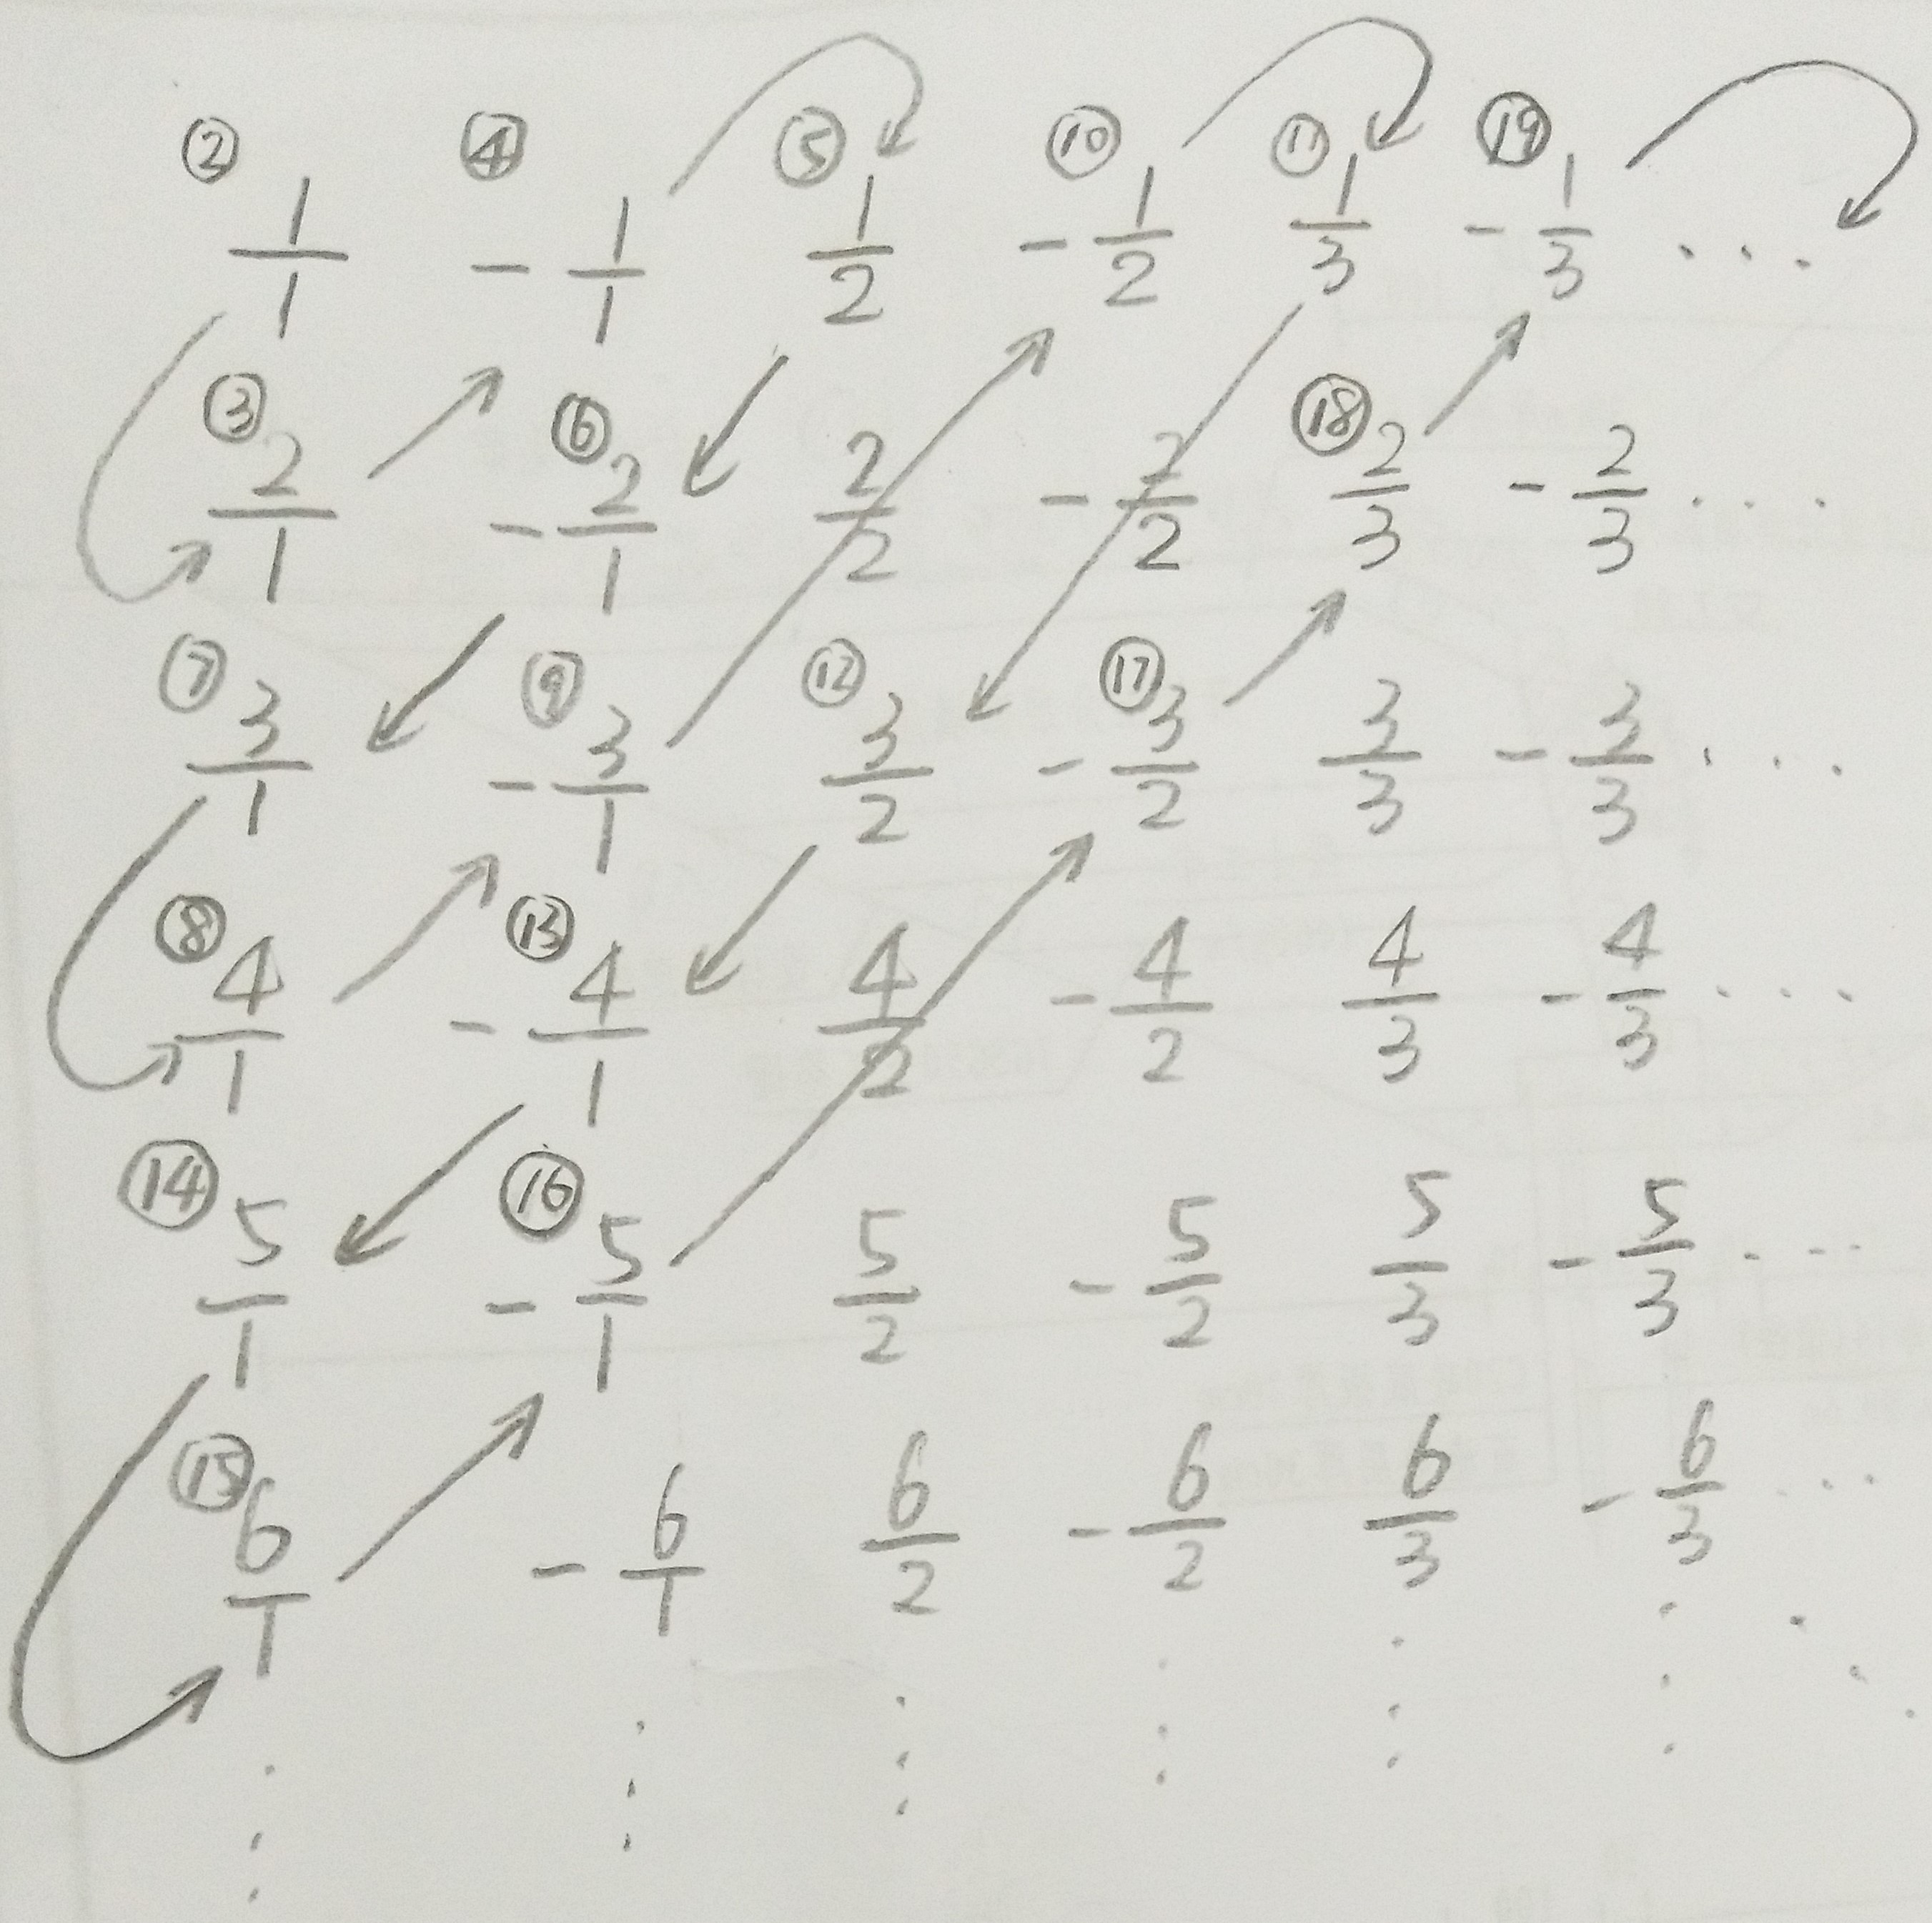
\includegraphics[scale=.15]{Homework_1Problem_9.jpg}
\caption{Problem 9} \label{Problem9}
\end{figure}
\end{sol}



%Copy the following block of text for each problem in the assignment.
\begin{problem}{10}
Let $A$ be the set of all sequences whose elements are the digits $0$ and $1$. For example, the following sequence is a element of $A$.
\[1,0,1,0,0,0,1,1,...\]Prove that set $A$ is uncountable. (Hint: You can prove it by using Cantor's diagonal process.)
\end{problem}
\begin{sol}
Suppose we associate every zero-one sequence in set $A$ with a unique natural number like the following list does:
\begin{align*}
0\rightarrow&a_{01},a_{02},a_{03},a_{04},......\\
1\rightarrow&a_{11},a_{12},a_{13},a_{14},......\\
2\rightarrow&a_{21},a_{22},a_{23},a_{24},......\\
3\rightarrow&a_{31},a_{32},a_{33},a_{34},......\\
......&
\end{align*}
where $a_{ij}=0$ or $1$.

Then we construct the following zero-one sequence through Cantor's diagonal process:
\[
b_0,b_1,b_2,b_3,......
\]
where
\[
b_i=\left\{\begin{array}{ll}
1,~~\text{if }a_{i~i+1}=0\\
0,~~\text{if }a_{i~i+1}=1
\end{array}\right.
\]

Obviously, sequence $b_0,b_1,b_2,b_3,......$ belong to set $A$. However, according to the definition of the $b_i$, there will always be at least one digit (the $i$th digit) different for sequence $b_0,b_1,b_2,b_3,......$ and sequence $a_{i1},a_{i2},a_{i3},a_{i4},......$. Here comes a contradiction. Therefore, we can not associate every zero-one sequence in set $A$ with a unique natural number, which means that set $A$ is uncountable.
\end{sol}












































































%%%%%%%%%%%%%%%%%%%%%%%%%%%%%%%%%%%%%%%%
%Do not alter anything below this line.
\end{document}